\documentclass[../memory.tex]{subfiles}

\begin{document}
\chapter{Planning}
The purpose of this chapter is to provide an overview of the planning,
organization, and development process of the frontend application. Planning
plays a vital role in ensuring time efficiency, making it essential to engage in
thorough planning before commencing development. Additionally, creating a
minimal user interface (UI) prior to the actual development phase can
significantly expedite the process.
\\
It is worth emphasizing that the planning stage should also allocate time for
thesis writing, as it constitutes an integral part of the overall project.
\section{Sprint planning}
When planning the work for the frontend project, our main goal was to avoid
being blocked by backend progress. It is common for frontend and native
developers to fall behind schedule because they are unable to progress until the
backend is complete. One solution to reduce this lag between frontends and
backends is to use GraphQL. However, in our case, we opted to apply GraphQL
ideas in a RESTful API, resulting in the following steps:
\begin{enumerate}[label = -]
	\item Defining the expected request body of a specific endpoint, in order to
	      let the frontend know \emph{what the service expects to receive}.
	\item Defining the response, if any, that an endpoint would return for a given call.
\end{enumerate}
This approach established a clear contract between the backend and the frontend,
with separated implementations that both parties agreed to respect.
\\
To facilitate development, we used a service worker to mock every API call made
in the local environment of a frontend developer. The service worker respected
the specified contract, allowing us to develop the frontend without being
blocked by the backend. Once the app was deployed, the service worker was
disabled, and the API calls were made to the \emph{actual} RESTful API. This
approach allowed for fast and non-blocking development for both frontend and
backend.
\\[8pt]
The second thing to take into account before starting to structure and develop
the frontend are the designs. Since there was not enough time to create a system
design and then enough designs that would cover all use cases of our app, we
opted for simple designs, which are shown in later sections. As a first sprint,
or sprint zero, I was in charge of prototyping the frontend application, which
would simplify the process of developing the frontend app.
\\[8pt]
Next steps are more involved in the development and architecture of the
application. As explained in previous sections, we got together every two weeks,
as well as keeping an asynchronous communication. We considered each meeting to
be a deadline, and in the meeting we would discuss the next steps to take or
changes if any. However, since there are always unexpected tasks, it has not
been easy to strictly follow the devised roadmap. The following diagram
illustrates an aproximate planning of the sprints.
\\
It is important to note that this initial planning is really subjective to
changes, as in any app development, there may be incidents, bugs, or other
issues that could temporarily block the development of the application.
Nonetheless, the goal was to stick as much as possible to the expected plan.
Also, Sprint 0 has not been added to the schema since it can be merged with the
tasks in the Sprint 1.
\begin{figure}[H]
	\centering
	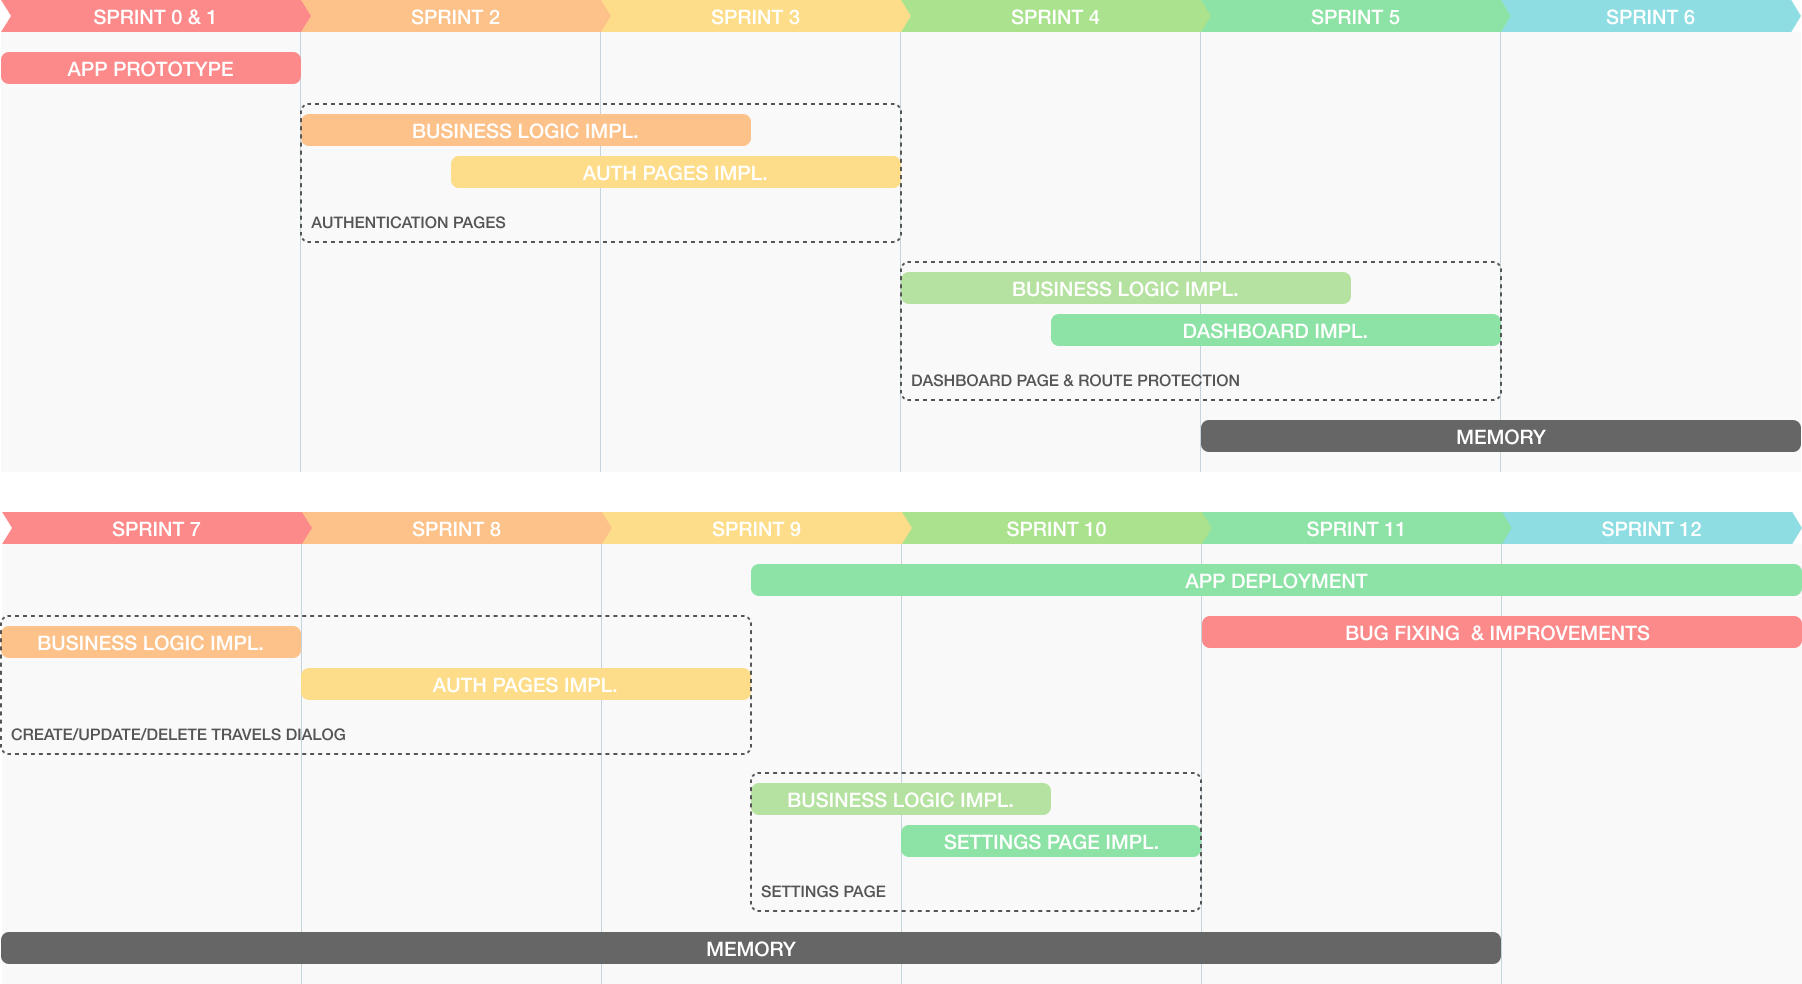
\includegraphics[width=\textwidth]{./assets/roadmap.png}
	\caption{Initial sprint planning}
\end{figure}
Aside from the Sprint 0 and 1 section, other sections consist of two weeks.
\section{Sprint development}
\subsection{Sprint 0 and 1}
As explained previously, the goal of the sprint 0 was to start prototyping the
application. Since there was no design system defined, it took a bit more than
two weeks to finish the prototypes, even though the were some part that would
change in a future.
\\
The design not only helped us visualise the entities and important parts of our
application, but also helped me architecture the monorepository. Once tool used
to simplify the developer experience is Nx. Using such build system, tasks as
having internal libraries and separated applications are easily handled.
Therefore, the goal of the sprint 1 was to set up the repository and have it
ready to roll. As I was defining the architecture of it, I was able to test
possible use cases that I could come across while developing the frontend. This
helped me prevent possible time-consuming issues, by handling them in an early
stage.
\\
One of the requirements for developing the application was to follow hexagonal
architecture patterns and domain-driven design. However, frontend frameworks and
technologies often deviate from traditional structures. For example, the React
framework primarily uses composition over inheritance and follows a reactive
paradigm. As a result, applying these concepts to the frontend posed a
significant challenge. More details about the final design will be provided in
subsequent chapters.
\subsection{Sprint 2 and 3}
Once the architecture was defined, the first goal of the sprint was to develop
the frontend domain logic for user sign up and sign in. As the first code
written for the core frontend, it was important to establish a solid structure
that could easily accommodate changes. The initial architecture planning proved
successful, with the following benefits:
\begin{enumerate}[label = -]
	\item The hexagonal architecture layers (domain, application, and
	      infrastructure) could be easily decoupled.
	\item The structure could be easily refactored and scaled as needed.
	\item The domain logic was separated from the frontend implementation, making
	      it reusable.
\end{enumerate}
Once the domain was defined and ready to be connected to a frontend application,
the next step was to implement the authentication pages. This process was
divided into two steps:
\begin{enumerate}[label = \arabic{*}.]
	\item Since most components had yet to be created, an initial implementation
	      was created in the respective package. This implementation was open to
	      modifications and designed to be reusable within different applications,
	      although it was already attached to the React framework.
	\item With the components created and the business logic defined, the last
	      step was to connect both through the view layer.
\end{enumerate}
Since there was not a lot of logic involved, it was possible to stick to the
original plan, and start developing the frontend views (log in and register
pages).
\\[8pt]
Once the logic architectue had been defined, the goal of the sprint was to start
developing the domain of the frontend that will contain the logic to sign up and
sign in a user. Being the first code written in the core of the frontend, it was
very sensitive to change in terms of structure. However, the initial
architecture planning turned out to work seamlessly well, this being:
\begin{enumerate}[label = -]
	\item Easily decoupling the diferent layers from the hexagonal architecture
	      (domain, application and infrastructure).
	\item Simplicity to escalate the context as well as to refactor it.
	\item Containing only business logic code, being completely unaware of any
	      frontend implementation, which allows such logic to be reused.
\end{enumerate}
Once the domain have been defined and was ready to be connected to a fronent
application, the next step was to start implementing the authentication pages of
the design. This process was divided in two steps:
\begin{enumerate}[label = \arabic{*}.]
	\item Most of the components had yet to be created, therefore an initial
	      implementation, open to modifications, was created in the respective
	      package. Note that, even though it is only used in one application, another
	      idea of the components internal library is that it can be reused within
	      different applications. However, it is already attached to a framework,
	      which, in this case, is React.
	\item Having the components created and the business logic defined, the last
	      step was a simple as connecting both through the view layer.
\end{enumerate}
Authentication pages require of a very basic layout, and most of the logic
happens in the form. However, as the logic had already been implemented in the
core package, such logic required only to be connected with the components.
Therefore, it simplified a lot the development of the view.
\\[8pt]
Initially it may not seem as an advantage, however if ever appeared the
necessity of developing another application that required the same logic, it
would mean that it could be reused. Therefore, the developers could only focus
in the implementation of the frontend, and then attaching the logic to it.
\subsection{Sprint 4 and 5}
For most of the tasks, to development of them involves a first implementation of
the business logic, a second part which may be optional which involves the
development of the required components, and a third one that is to involves
applying the logic to the view.
\\[8pt]
Similar to the authentication pages, the first task of the dashboard page
involved creating the initial travel mode. In the dashboard page, the user can
see a list of travels and interact with them. The interaction or management
would be later developed. The travel model is quite complex, as it is
fetched from the backend in a specific model, meaning that it should be parsed
and transformed to the expected object.
\\
Another setback that appeared during the development of the logic for the
dashboard was the travel model changes, which implied having to add, update or
delete all fields that differed. As some parts of the dashboard already included
the usage of the intial proposition of the travel model, the specific parts had
to be updated.
\\[8pt]
This exposed one of the common problems between the core package and the
frontend implementations that use that package. Any breaking change in the core,
as it is the updation of a model, can generate side-effects to the frontend that
depends on it. Knowing this issue, I came up with two solutions:
\begin{enumerate}
	\item First would be to create a versioning of the packages, meaning that the
	      frontend would depend on a concrete version of the core package. At start it
	      could be a good solution, yet it can be really easy to start leaving
	      frontends outdated. The update of the frontend is not inevitable, but it
	      would allow the team to update the changes in the main branch, and migrate
	      each frontend step by step.
	\item Second would be to work in feature branches, meaning that for every
	      breaking change in the core package, all the affected applications would be
	      updated accordingly. This implies that the team would have to focus on the
	      migration in order to accept the new changes.
\end{enumerate}
In this case, second option was chosen as versioning the packages was not
something planned from the starting point and, even though it is possible to be
added, updating all frontends was more simple. Additionally, only one
application had to be updated.
\subsection{Sprint 6}
In the sixth sprint, the team agreed to focus in writing the common parts of the
memory for the thesis. The goal was to finish as soon as possible such common
parts and later start writing non-common parts.
\\
Even though it was not a complex part, the team required of more coordination
than usual to start writing the common parts. A part or some parts were assigned
to each member, and a shared Google Docs containted all the parts.
\\
After a groupal revision, a couple of changes needed to be made, meaning that
the memory common parts task would expand to more that the one sprint, as
initially planned.
\subsection{Sprint 7 and 8}
These sprints were planned to be focused on the development of the travel
management from the frontend. However, as a team we agreed to \emph{push} the
memory and finish the common parts as soon as possible. This resulted in
stopping the development of the frontend temporarily.
\\[8pt]
Once the common part had been written or more advanced, the team could focus
back on the development. As explained in any previous task, first came the
modelling of the alerts. Inside the core package, there was already a lot of
business logic for the alerts, which required only to be extended by adding the
possibility to create, update and delete the travels.
\\
Next, only a couple of components were created or required
modification/extension. Inputs, buttons, text and so on had already been created
as were required by the other tasks.
\\
Finally, the connection between the logic and the frontend components. In
further chapters it will be explained in more depth, yet this tasks also require
a bit of state management. The library used to manage API calls and caching such
calls is also used as a state management solution. This helps reduce the logic
to be implemented in the core application, as it can be kept stateless.
\\
All this tasks include the respective testing, both in the core and in the UI
components.
\\[8pt]
Even though the development of this sprint seems really straightforward, it
included more frontend logic than the other tasks. Basically, any action
(creation, updation or deletion) of an alert should update the dashboard table.
However, as a commonly known problem in React it is the amount of rendering that
must be done, for any state changes. This topic will be explained in later
chapters, yet the architectural decisions that impacted performance were made
during this sprints.
\subsection{Sprint 9 and further}
As the memory took up part of the previous sprints, it was at this point that
the initial planning started to tumble. As explained in the beginning, the
roadmap was just an idea to align with the rest of the team on what to focus.
Nonetheless, during the majority of the time, it was possible to stick to the
roadmap.
\\[8pt]
The management of travel tasks required more time for full development,
resulting in an underestimation of the total workload. As a result, these tasks
were not resolved until the 12th sprint. Another factor contributing to the
extended time required was the simultaneous development of the automated
application deployment process. This deployment is a critical task as it allows
access to the MVP outside of the local development environment. Additionally, as
a team, we needed to ensure that all connections, from the frontend application
to the backend application, functioned seamlessly.
\\[8pt]
With all this in mind, there was very little, to any time to develop the
settings page. Also, since there was no service nor endpoint to update the user
settings (also because of time constraints), such task was not developed.
\\
Furthermore, end-to-end tests were also skipped because of time constraints.
\end{document}
